\section{古诗文写作助手}\label{sec-7}
\subsection{数据集与预处理}
为了构建一个能够有效生成古典诗词的大语言模型,我们小组选择了来自GitHub上的公开数据集\textit{Chinese-Poetry}作为训练基础。该数据集由同名项目维护,网址为:\url{https://github.com/chinese-poetry/chinese-poetry},涵盖了中国古代文学的广泛领域,包括但不限于诗、词、曲等多种体裁。
    
考虑到模型的特定应用目标——即专注于古诗词的生成——我们在初步的数据收集阶段进行了针对性的选择。具体来说,我们从原始数据集中筛选出了以下几类具有代表性的古诗词条目,以确保数据集的纯净度和相关性:
\begin{itemize}
    \item 曹操诗集:收录了三国时期曹操创作的诗歌作品。
    \item 楚辞:战国时期的楚国诗人屈原等人的抒情长诗。
    \item 纳兰性德:清代著名词人纳兰性德的作品集。
    \item 全唐诗:唐代诗歌的汇总,几乎囊括了所有流传至今的唐诗。
    \item 诗经:中国最早的诗歌总集,包含西周初年至春秋中期的诗歌。
    \item 水墨唐诗:精选唐代诗歌,侧重于描绘自然景观和社会生活。
    \item 宋词:宋代词作的集合,展现了宋朝文人的艺术风采。
    \item 五代诗词:涵盖了五代十国时期的诗歌创作。
    \item 御定全唐诗:清朝康熙年间编纂的官方版唐诗全集。
    \item 元曲:元代戏曲剧本中的唱词部分,体现了当时的文化特色。
\end{itemize}
    
在数据预处理阶段,我们进一步优化了数据结构,以便更好地服务于模型训练的需求。我们的目标是创建一个简洁而易于处理的文本文件(.txt),其中每首古诗词的标题和内容被整合在同一行内,采用“标题:内容”的格式。例如:
\begin{verbatim}
日诗:欲出未出光辣达,千山万山如火发。须臾走向天上来,逐却残星赶却月。
\end{verbatim}

这一过程不仅简化了输入格式,提高了训练效率,还减少了不必要的数据冗余,使得后续的文本处理步骤更为直观易行。最终,经过清理和格式化后的数据被保存为文本文件(.txt),以供模型训练使用。
\subsection{模型训练与封装}
在实现了基本的Transformer架构下的诗词生成器之后,我们接着尝试将其封装为诗词创作助手。此时我们已经不再满足于基本的诗词创作或者是仅仅根据提示词返回有关系的上下文,我们更希望其能够在用户设计的一定的格式要求下(比如创作方式、是否押韵、平仄变化等等)尽可能创作出丰富多变的内容,这实际上提出了远超基本Transformer架构诗词生成其的功能,在这个过程中也遇到了一系列问题和挑战。

以下我们先对模型封装进行简单的介绍,然后介绍核心推理模式与基本逻辑,之后介绍助手设计,最后展示实现效果。

在之前的内容中我们实现了模型的训练、保存、读取和简单的推理指令。我们不能严格控制每次输出的长度,只能给予其长度上的最大限制。同时我们也注意到,在多次重复实验中,模型推理产生的文本标点符号的出现规律并不严格遵守规则。

以唐诗为例,我们在多次重复实验中出现短句长度不一的情况,这一方面是我们的训练文本本身包括了大量长度不同、规制各异的诗句,另一方面是我们在推理中引入了部分随机性所致。此时的我们考虑的两种解决方案一是增添数据预处理环节,针对不同长度不同规制的诗句训练不同的模型,同时放弃引入随机性,但这可能与“创作”的概念相违背。因此我们考虑了第二种方案,在保持当前模型的自由性的前提下,靠外部函数对推理内容做筛选和整理。

同时因为我们找到了部分词和元曲的数据,我们也进行了数据提取、模型训练和模型推理,但现实中词和曲的创作规则过于复杂,难以通过简单的逻辑描述完备,因此我们仅对其实现了完全自由的创作模式。其实现效果并不是特别好,词中可能出现过长或者过短的句子,而元曲中复杂的标点符号的使用逻辑和并不常规的言语表达都可能造成歧义,但整体来说,诗、词、曲仍然展示出了完全不同的风格和内容。

首先,我们对模型训练功能进行了封装(\texttt{trans\_poem.py}),使之能够接收外部输入参数\texttt{data\_path},从而提取当前文本的命名关键词。根据所处的训练环境,该模块自动生成适用于GPU和CPU两种版本的模型,并最终返回训练好的模型及相应的词典。

其次,针对模型推理功能的封装(\texttt{assistant.py})实现了对外部指令的响应能力,如创作题材的选择、是否提供关键词、是否考虑平仄与押韵等特性。此模块能够自动选择合适的模型、词典以及推理函数来执行推理过程,并最终反馈能否实现用户要求及具体的推理结果。

最后,在\texttt{main.py}中调用推理功能,在操作台读取交互过程中产生的更符合用户习惯的命令,以返回生成的诗词内容。我们也额外设计了简易的UI界面,运行\texttt{peomUI.py}即可实现,这更便于在生成失败后进行提醒和连续多次生成。

\subsection{核心推理模式与基本逻辑}
在进行诗的生成时,我们主要考虑以下几点问题:是否由用户指定主题、生成的模式是“创作”还是“续写”、是否指定句数和句长、是否要符合平仄、是否要押韵。接下来我们将逐个介绍其逻辑是如何影响推理的。

首先,为了能够在推理中引入随机性,我们编写函数让每次推理仅生成一个字符。这个字符是可能包含标点符号的,确实存在某些汉字与逗号、句号建立了比较强的关系,可以证明其经常出现于句末。我们收集至多一个固定上限的结果,并从中抽取一个汉字作为推理结果,这可以让一个模型根据同样的提示词生成完全不同的结果,符合“写诗”的概念,我们暂时称其为“基本推理”模式。于此同时,我们也设计了将收集结果打乱后全数返回的推理模式,我们称其为“严格推理”模式,这两个模式都在复杂的用户需求中发挥了不同的作用,这也是我们实现写作助手功能的核心。

句数和句长为推理结果限制了基本的输出范围,并在合适的位置添加标点符号,默认为4句七言诗。平仄的规律则相对来说更多样,比如五言诗“平平仄仄平”“仄仄平平仄”,七言诗“平平仄仄平平仄”等等,而且由于部分汉字的读音已经随时间变化以及一字多音的情况,我们无法对平仄进行精细的设计,因此我们考虑借助python中的pypinyin库对汉字读音进行判断,一声为“平”,其余为“仄”,推理限制为不能连续出现三“平”或者三“仄”。押韵即在每个短句生成结束时判断偶数句尾的汉字韵母是否一致,在这里我们也暂时不考虑平翘舌带来的语感不一致问题,比如“日”“期”二字韵母相同但语感上并不押韵。平仄和押韵可以同时要求,但现实中同时满足这两个条件的诗句也相对较少。

创作模式即根据主题词创作相关内容,主题词本身并不一定会出现在句中。用户也可以并不提供主题词,会自动从字典库中抽取汉字作为主题词。续写模式即接受不长于设定句长的主题词后进行推理,生成诗句开头一定是主题词。这两个模式对目标向量(src和tgt)做出了不同的切分处理。除此之外还需要考虑,续写的推理逻辑需要保证连贯性并在句末插入“停止”,这样可以避免生成结果在实质上等同于“一句连续的话强行断开”;而主题创作的推理逻辑需要保证内容始终围绕关键词,在每句话成功生成后都要重新返回关键词附近进行推理。

\subsection{助手设计}
在之前的介绍中,我们已经介绍了两种保证一定随机性的推理模式,接下来我们结合平仄和押韵的设计来介绍它们的用途。根据用户是否选择平仄和押韵,实际上可以分为四种模式,但是由于他们实际上是在不同生成位置进行的的检测,因此我们可以分开设计,在必要的位置根据实际情况合并即可。

如果用户完全没有任何要求,那么仅需启动基本推理模式,实现多样的输出即可。平仄的设计需要在一句生成每个汉字时检测其读音,并与前若干个字符进行比较,如果出现了连续三个“平”或者“仄”,基本推理模式可能会多次返回相同的选择,造成死循环,因此我们需要严格推理模式,通过对结果集中的字符逐个尝试尽可能快速找出合适的字符。如果遍历整个结果集仍不能找到合适的字符,就返回生成失败的提示。但经过实际测试这种情况发生的概率较低。押韵的实现也与此类似,如果在一句话生成完毕后发现最后一个字不押韵,那么就在结果集中遍历寻找符合要求的字重新加入,找不到则提示用户尝试修改要求。

如果需要同时满足平仄和押韵,先在逐字生成时尽可能满足平仄要求,当一句话生成结束时检测最后一个字是否押韵,如果不符合要求则在结果集中寻找同时满足两个条件的字,找不到则优先满足平仄,并提示用户尝试修改要求。值得注意是,在续写模式下,如果用户提出了平仄需求,需要对用户的输入进行检测,发现错误则提示用户输入不满足平仄要求。

随机推理也会带来一定坏处,比如有可能会加速一句话的“结束”,可能会出现现代汉语中的生僻字,在更严苛的条件下这种情况发生的概率也越高。如果我们检测到当前这句话的长度不满足要求,则会在一定次数上限内不断尝试生成这句话,如果仍不能正确生成则提示用户尝试修改要求。如果觉得目前的失败触发概率过高,也可以通过修改\texttt{assistant.py}中内置参数tolerance来提高严格推理的词集容量上限,这为诗句生成提供了更丰富的可能性,大大降低失败的概率,但相应地也会提高响应时间。

总的来说,我们建议使用的时候尽可能提出较低的平仄和押韵要求,同时设置较短的句长,这会大大提高文本的生成成功概率和质量。为了能够在每次生成诗句时快速响应,根据用户的输入要求,助手会启用不同的推理函数,每个推理函数内已经设计好了结合给定参数的推理流程,这样可以尽量减少判断和循环,示意图\ref{fig:iwslt-wmt3}如下所示。

\begin{figure}[h]
    \centering
    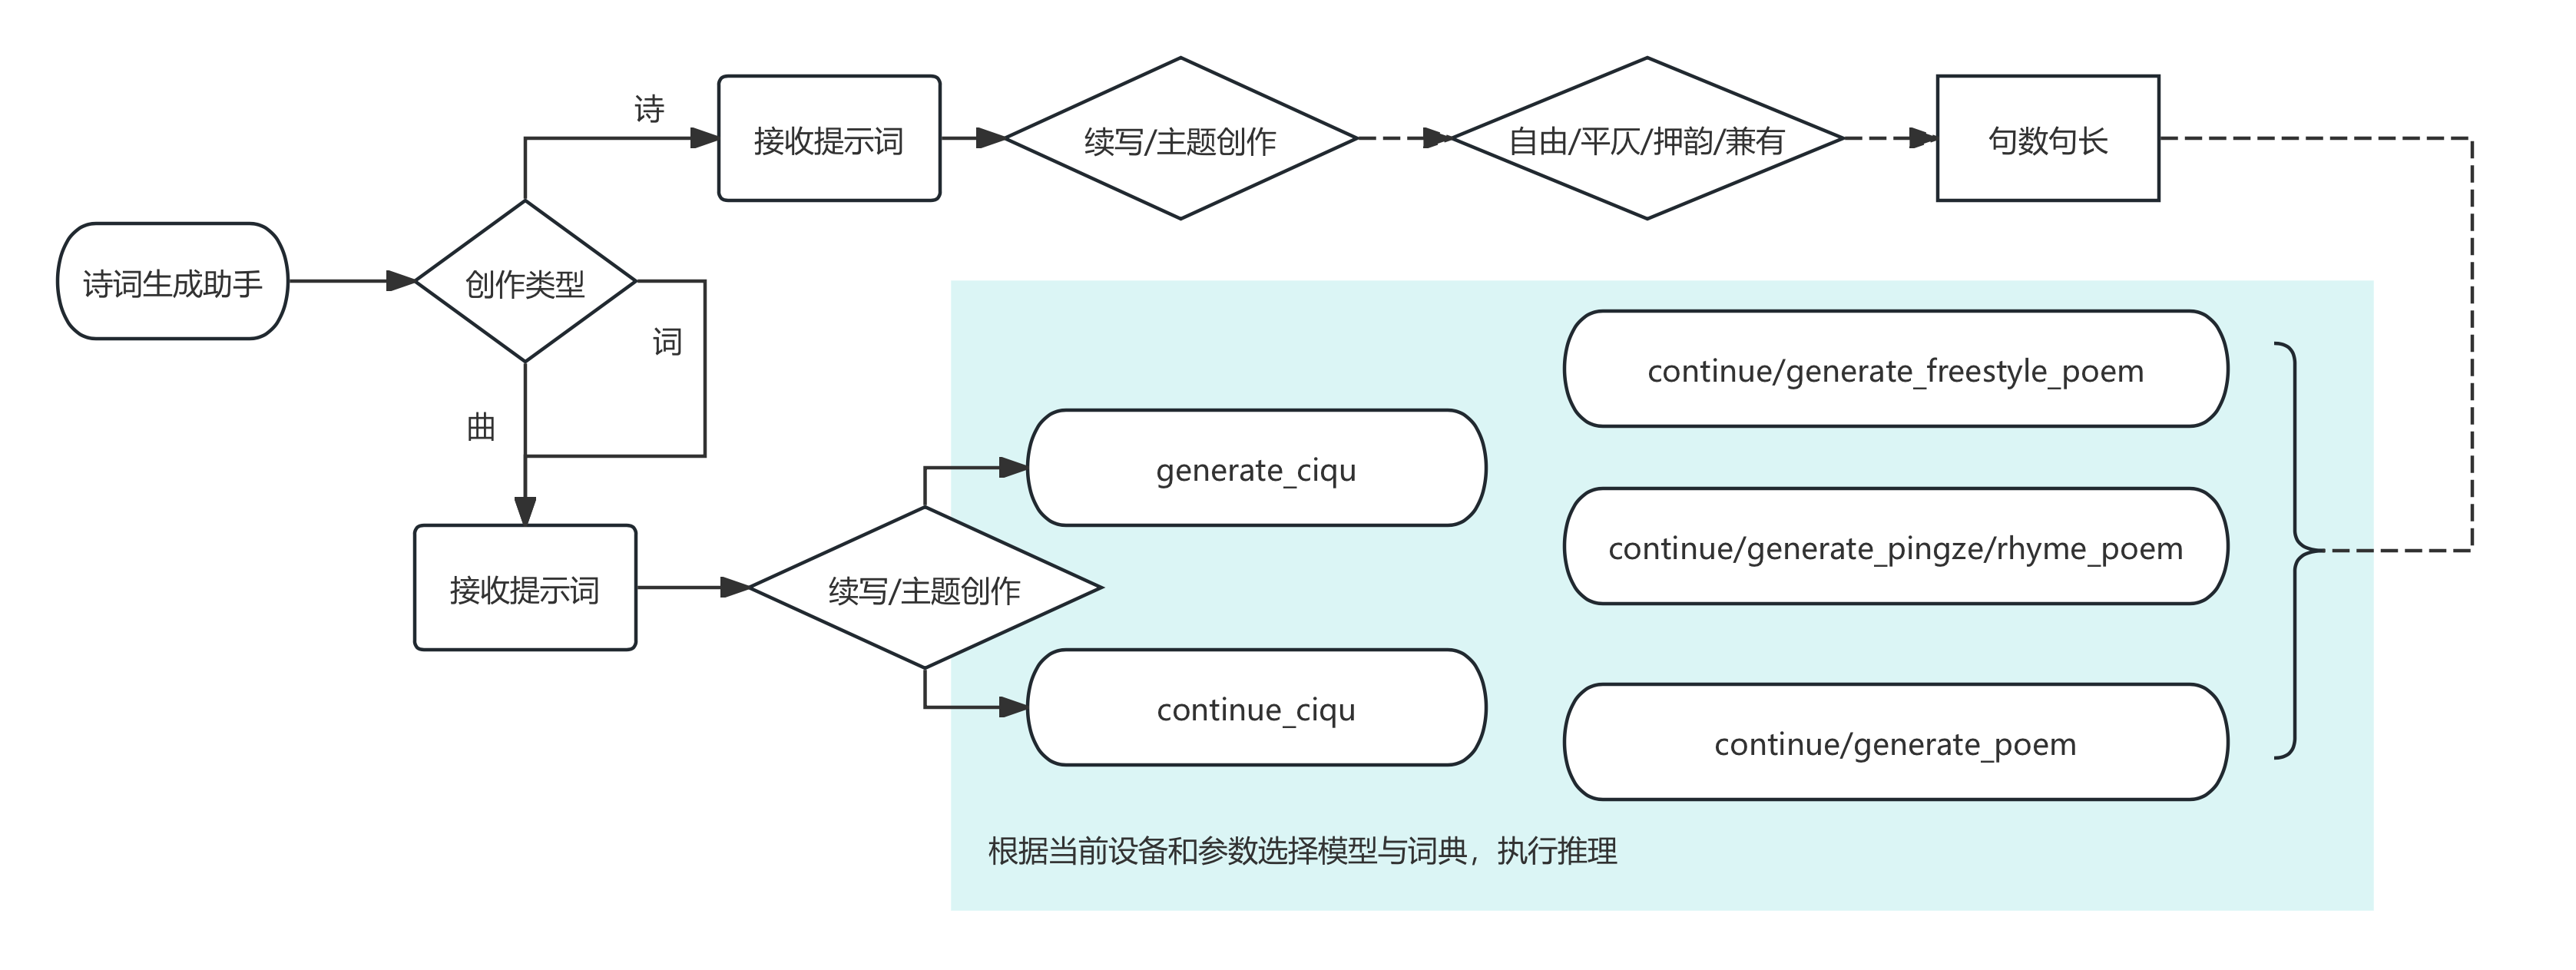
\includegraphics[width=\textwidth]{img/wirter/诗词生成助手流程.png}
    \caption{诗词生成助手外部流程示意图}
    \label{fig:iwslt-wmt3}
\end{figure}

\subsection{实现效果}
\textbf{操作台执行结果}
\begin{figure}[h]
    \centering
    % 第一个图像
    \begin{minipage}[b]{0.44\textwidth}
        \centering
        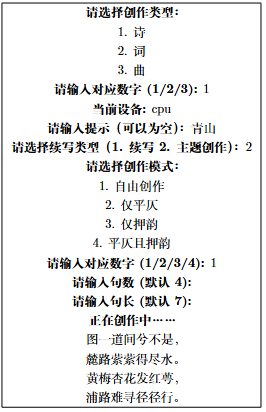
\includegraphics[width=\textwidth]{img/writer/操作台执行结果.png}
        \caption{操作台执行结果}
        \label{fig:operation_result}
    \end{minipage}
    \hfill
    % 第二个图像
    \begin{minipage}[b]{0.49\textwidth}
        \centering
        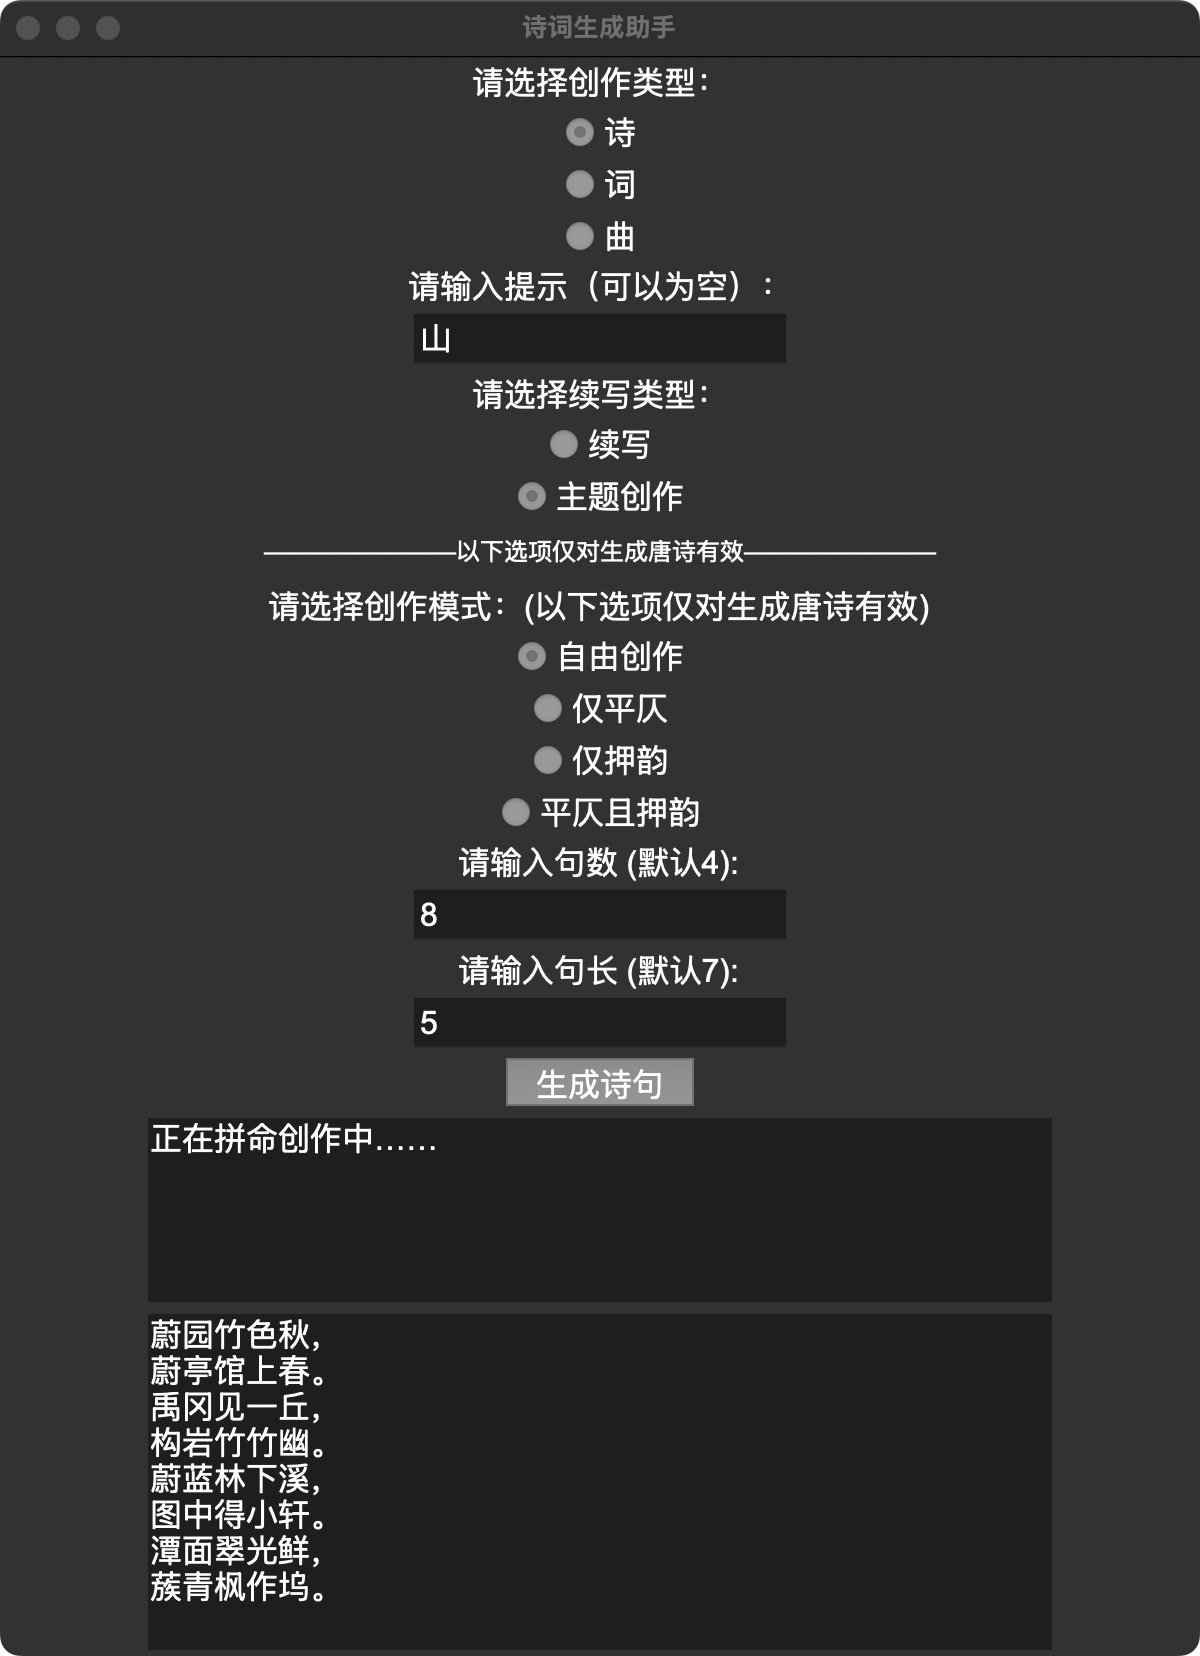
\includegraphics[width=\textwidth]{img/writer/结果1.jpg}
        \caption{诗词生成助手运行展示}
        \label{fig:poem_generator_demo}
    \end{minipage}
\end{figure}
